\section{Methodik}

\subsection{Möglichkeiten der Datenerfassung}
Dieser Abschnitt beinhaltet verschiedene Ansätze, wie die Daten vom Wandler abgerufen werden können. Dies beinhaltet die Verwendung eines PICkit Serial Analysers sowie die eines Raspberry Pi.


\subsubsection{Notwendigkeit eines Pegelwandlers}
Dadurch bedingt, dass der verwendete Wandler einen Pegel von fünf Volt am I²C Bus besitzt, und ein Raspberry Pi jedoch nur 3.3 Volt, ist es notwendig einen Pegelwandler zwischen die beiden Platinen zu schalten. Der dabei verwendete Pegelwandler von der Familie TXB01.

\subsubsection{PICkit Serial Analyzer}
Das Aufzeichnen der Wandler-Daten kann innerhalb zweier Plattformen durchgeführt werden. Eine Plattform ist hierbei ein PICkit Serial Analyzer, der es ermöglicht, auf einem Windows Betriebssystem unter der Verwendung der Programmiersprache C# \hl{Das I²C Protokoll} zu betreiben. Der genannte Serial Analyzer ist in Abb. \hl{X} zu erkennen. Dieser besitzt, wie in der Markierung 6 zu sehen ist mehrere Anschlüsse, welche für verschiedene Protokolle wie I²C, UART und SPI verwendet werden können. Der Quellcode, welcher zur Datenerfassung per PICkit verwendet wurde, ist im \hl{Anhang zu finden}. Der Ablauf des Programms beginnt mit der Definierung verschiedener Funktionen um aus Byte-Daten die tatsächlichen Werte zu berechnen. In der Main Funktion werden zu beginn alle relevante Programmparameter definiert und initialisiert. Dies schließt Adressen, Datenarrays sowie Konfigurationsparameter des PICkit mit ein.  Anschließend erfolgt die Initialisierung des PICkit mit den vorher definierten Parametern. Abgeschlossen wird das Programm durch einen superloop, welche kontinuierlich Daten vom Wandler ausliest, auswertet und in eine Datei abspeichert. \hl{Evtl. noch die Codezeilen mit angeben}

\begin{figure}[H]
    \centering
    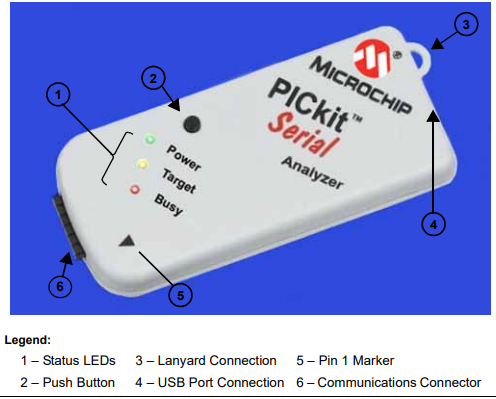
\includegraphics[height= 9cm, width = \textwidth]{Pictures/pickit.png}
    \caption{Strukturierung der gemessenen Daten}
\end{figure}


\subsubsection{Raspberry Pi}
Die zweite Plattform, welche in den Folgenden Tests primär genutzt wird, ist ein Raspberry Pi. Dadurch, dass einem Raspberry Pi sowohl I²C Pins als auch entsprechende Software Libaries zur Verfügung stehen, ist es möglich auch darauf das I²C Protokoll zu nutzen.\\

Es ist ebenfalls wichtig erwähnen, dass die Struktur, in der die Daten innerhalb der Software abgefragt werden relevant ist, da diese sowohl die Abtastrate, als auch die Qualität der Daten beeinflussen kann. So zeigt die Variante 1 des Codes im Anhang eine mögliche Struktur. In dieser werden die einzelnen Parameter separat nacheinander in 2 Byte Blöcken abgefragt. Dies hat den Vorteil, \hl{das die Daten spezifisch abgefragt werden können}. Die Nachteile dieses Verfahrens sind jedoch, ein zusätzlicher Overhead, da durch mehrmaliges Abfragen jedes mal die Adresse des Mikrocontrollers mit angegeben werden muss, was den Datenfluss verlangsamt. Das bedeutet, dass die Adressbits, welche in Abb. \hl{3} dargestellt sind, mit jeder Abfrage mitgeschickt werden müssen. Ein weiterer Nachteil ist, dass die Daten nicht vom selben Zeitabschnitt stammen. So werden beispielsweise, während die Daten aus dem Temperatur Register abgefragt werden, bereits die Daten in den Spannungs- und Stromregistern aktualisiert. \\
\\
Die Abfragestruktur, welche zu bevorzugen ist, ist im Anhang als Variante 2 dargestellt. Diese zeigt, dass alle 8 Bytes des Datenregisters auf einmal ausgelesen werden. Dies hat den Vorteil, dass alle Daten zur gleichen Zeiteinheit abgefragt werden und verhindert zugleich den o. g. Effekt des Overhead, da alle vier Datenregister mit einmaligem versenden der Adresse abgerufen werden. 


\subsection{Speicherung und Strukturierung der Daten}
Die Speicherung der erfassten Daten erfolgt während der Programmlaufzeit. Dieser Umstand bietet sowohl Vor- als auch Nachteile. Ein Nachteil dieser Strategie ist, dass das speichern der Daten nach jeder Abfrage Rechenzeit kostet, was die Abtastrate des Systems verlangsamt. Ein Vorteil dieser Methodik ist jedoch, dass Daten sofort gespeichert werden, und somit nicht die Möglichkeit besteht, dass die Daten bei einem Programmabsturz verloren gehen. Ein weiterer Vorteil besteht darin, dass die Daten nicht im RAM des Raspberry Pi gespeichert werden müssen, da sie mit jeder neuen Datenabfrage auf der Festplatte gespeichert werden, und die Daten im RAM sofort von neuen Daten überschrieben werden. Zusammengefasst kann gesagt werden, dass eine geringe Beeinträchtigung der Abtastrate in kauf genommen wird, für eine geringere Auslastung des RAM und mehr Sicherheit bei der Datenerfassung.

In Abb. \hl{x} ist der Ausschnitt eines Datensatzes zu erkennen. Die Spalten repräsentieren jeweils eine Kategorie von Daten, wie z. B. die Temperatur. Die einzelnen Zeilen beinhalten jeweils einen kompletten Datensatz, welcher in der Zeit aufgenommen wurde, der im Zeitstempel eingetragen ist. Der Zeitstempel hat das Format Stunden:Minuten:Sekunden:Millisekunden.

\begin{figure}[H]
    \centering
    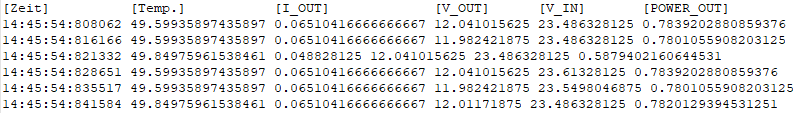
\includegraphics[height= 2.5cm, width = \textwidth]{Pictures/dat_struct.png}
    \caption{Strukturierung der gemessenen Daten}
\end{figure}



\subsection{Methoden der Datenverarbeitung}
In diesem Abschnitt werden die einzelnen Methoden der Datenverarbeitung innerhalb der Software dargestellt. Dies beinhaltet das Laden der Daten, das preprocessing sowie die Visualisierung. Das Laden der Daten erfolgt in der Funktion "unr\_data", welche im Anhang in der Sektion \hl{x} gefunden innerhalb der Zeilen 70 und 117 gefunden werden kann. In dieser Funktion werden die Daten, welche in einer Textdatei gespeichert sind, in eine Matrix gespeichert, welche durch die Library "Numpy" generiert wird. Nachdem die Daten geladen wurden, muss im nächsten Schritt der Zeitverlauf aus den Zeitstempeln generiert werden. \hl{Dies ist deshalb notwendig, da die Daten nicht mit dem Zeitformat "\%H:\%M:\%S:\%f" visualisiert werden können. Aus diesen Zeitstempel werden Zeitdaten in Sekunden generiert.} Sobald die Zeitstempel formatiert wurden, gibt die Funktion in Zeile 117 eine Matrix mit den gemessenen Daten und ein Array mit dem Zeitverlauf aus. Was ebenfalls zu erwähnen ist, ist die For-Schleife am Ende der unr\_data Funktion. Diese Schleife dient dazu Fehler in einem rudimentären Ausmaß zu erkennen. Wie in dem Code zu erkennen ist, werden Datenwerte, welche kleiner als null und größer als Hundert sind als Fehler gehandhabt und können entweder nur zu einem Fehlerzähler hinzu-addiert werden oder direkt dadurch kompensiert werden, indem anstelle des Fehlerhaften Werts der vorher kommende Wert verwendet wird.

Dadurch bedingt, dass alle Signale rauschen, existiert die Möglichkeit einen Software-gesteuerten Tiefpassfilter über das Signal zu legen. Diese Funktion ist zwischen den Zeilen 120 und 125 in der Funktion "apply\_filter" zu erkennen. Diese Funktion kann über die Library "scipy" genutzt werden. 

Eine weitere wichtige Funktion ist "calc\_meta". Diese Funktion dient dazu Metadaten des vorhandenen Datensatzes zu berechnen. Zu den Metadaten gehören: Mittelwert, Länge des Datensatzes, Standardabweichung, numerische Minimum- und Maximum-Werte. Dadurch, dass als Input-Parameter die gesamte Datenmatrix übergeben wird (data), ist die Ausgabe entsprechend eine Matrix in der zu jedem Datensatz (Strom, Spannung, Temperatur) ein Array mit den Metadaten gehört.

Alle bisher genannten Funktionen können genutzt werden, um die Daten abzurufen und zu visualisieren, wie in \hl{den Zeilen} 158 bis 168 aufgezeigt ist. Es werden Daten aus jeder Datei in einem Verzeichnis geladen, Metadaten berechnet sowie ein bestimmtes Signal visualisiert werden.



\subsection{Statische Datenerfassung}

Die statische Datenerfassung dient dem Zweck, die Funktionalität der Wandler unter einer konstanten Last zu überprüfen. Es wurden zwei simple Testfälle aufgebaut. Bei beiden handelt es sich um Parallelschaltungen von 4,7 Ohm Widerständen. Der erste Fall schaltet zwei davon parallel, der zweite drei. Durch das Anwenden des Ohmschen Gesetzes, kann ein theoretischer Stromfluss und somit auch die theoretische Leistungsaufnahme berechnet werden. Der Wandler wird durch ein Netzteil mit 24 Volt Ausgangsspannung betrieben. Diese 24 Volt werden von dem Wandler auf 12 V herabgesetzt. Somit kann der Strom berechnet werden, der durch die Widerstände fließt. Bei zwei parallel-geschaltenen Widerständen ergibt das einen theoretischen Stromfluss von 5.1 A wie und bei drei parallel geschaltenen Widerständen 7.65 A wie in den Gleichungen 3 und 4 zu sehen ist.

\begin{equation}
\label{Ohmsches Gesetz}
\frac{U}{R} = I \tab
\end{equation}


\begin{equation}
\label{Ohmsches Gesetz}
\frac{12V}{4.7 \ohm}*2 = 5.10 A 
\end{equation}


\begin{equation}
\label{Ohmsches Gesetz}
12V*4.7 Ohm*3 = 7.65 A 
\end{equation}


Da die statische Datenerfassung über eine konstante Last durchgeführt wird, sind hohe Abtastraten nicht zwingend erforderlich. Aus diesem Grund ist die Nutzung eines PICkit, welcher eine geringe Abtastrate besitzt \hl{nicht problematisch}. Es wird jedoch trotzdem ein Raspberry Pi zur Datenerfassung verwendet, da dieser durch seine höhere Abtastrate eine feinere Ansicht der Daten ermöglicht, wodurch das Rauschen der Daten \hl{besser dargestellt werden kann}. 

\subsection{Dynamische Datenerfassung}

Das Ziel der dynamischen Datenerfassung ist es, zu evaluieren, wie der Wandler sich unter Lasten verhält, die sich mit der Zeit ändern. Sowie mögliche Abweichungen zwischen den einzelnen Wandlern selbst. Der Testaufbau beinhaltet den Hybridwandler, einen Stereoverstärker, welcher per Wandler mit Strom versorgt wird und in den ein Audiosignal eingespeist wird. In Abb. 5 ist die Schaltung des Testaufbaus abgebildet. Es ist zu erkennen, das am Eingang des Buck-Wandlers 24 V eingespeist werden und das die am Ausgang liegenden 12 V an den Stereoverstärker angeschlossen sind. Des Weiteren ist ersichtlich, dass nur ein Kanal des Stereoverstärkers genutzt wird. Dieser Kanal wird mit einem Audiosignal aus einem externen Rechner versorgt. Als Signale werden hierbei Sinussignale mit variierender Frequenz verwendet, welche mit dem Programm Audacity generiert werden. Das Ausgangssignal fällt über einen Lastwiderstand ab. Obwohl es ein Stereoverstärker ist, wurde auf einen Lautsprecher verzichtet, da durch einen Lastwiderstand die Reproduzierbarkeit gewährleistet wird. 


\begin{figure}[H]
    \centering
    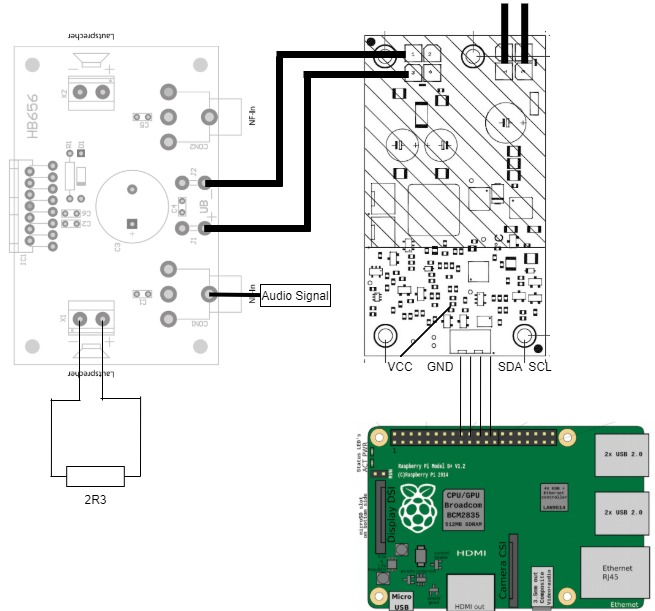
\includegraphics[height= 8cm, width = \textwidth]{Pictures/Dyn_Schaltung.jpg}
    \caption{Versuchsaufbau der dynamischen Datenerfassung}
\end{figure}

Der erste Testschritt ist dabei die Überprüfung, wie hoch die maximale Frequenz eines Signals sein kann, sodass interpretierbare Daten erzeugt werden können. Die maximale Frequenz kann durch praktische Tests empirisch bestimmt werden. Der Umfang dieser Tests besteht darin, die Daten von mehreren Wandlern über einen Zeitraum T zu messen und anschließend die Anzahl der gemessenen Samples durch die gemessene Zeit zu teilen, um so die durchschnittliche Sample-Rate pro Sekunde zu erhalten. 

Dadurch, dass die Datenerfassung auf einem Raspberry Pi abläuft, ist es möglich, die Daten nach jeder Abfrage sofort in eine Textdatei abzuspeichern. Es werden Daten zur Zeit, Temperatur, Ausgangsstrom, Ausgangsspannung und Eingangsspannung aufgezeichnet und tabellarisch abgespeichert.

Die Nyquist-Frequenz stammt aus der Signaltheorie und setzt die maximale Abtastrate in Verhältnis mit der maximalen Frequenz, die ohne Verzerrungen dargestellt werden kann. Die Gleichung besagt, dass die maximale Frequenz, die ohne Verzerrungen dargestellt werden soll, mit einer Abtastrate abgetastet werden soll, die mindestens doppelt so hoch ist, wie die abgetastete Frequenz. Sobald die Abtastrate experimentell bestimmt werden kann, kann das Nyquist-Frequenz theorem darauf angewendet werden, um so die Frequenz zu bestimmen, die maximal mit dem Wandler abgetastet werden kann. 


\subsubsection{Echtzeitmonitoring}
Das Ziel des Echtzeitmonitoring ist es, in laufenden Betrieb des Wandlers Daten zu Strom, Spannung und Temperatur zu erheben, diese Daten zur Verarbeiten und Aussagen darüber zu treffen, welche Last gerade an dem Wandler angeschlossen ist. Eine Last ist in diesem Fall ein Audiosignal, welches durch einen Stereo Verstärker, welcher an den Wandler angeschlossen ist, verstärkt wird. 
Zur Klassifizierung, welche Last, bzw. welches Signal gerade am Stereoverstärker angeschlossen ist, wird ein neuronales Netz verwendet, welches per Tensorflow API generiert wird. Die gemessenen Signale werden dann vom Raspberry Pi, zwecks Verminderung der Rechenleistung, per Socket an einen Rechner geschickt, welcher dann die Daten per Neuronales Netz interpretiert und eine entsprechende Klassifizierung berechnet. Als Testfälle wurden Sinussignal mit verschiedenen Frequenzen verwendet, um die allgemeine Anwendbarkeit von Deep-Learning Algorithmen zu verifizieren. 

\subsubsection{Vergleichsmonitoring mehrerer Wandler im laufenden Betrieb}
Das Ziel des Vergleichsmonitoring ist es, eine Software Struktur aufzubauen, welche es ermöglicht, mehrere Wandler gleichzeitig auf einem Raspberry Pi per I²C zu betreiben und die Daten in Echtzeit zu visualisieren und in Textdateien abzuspeichern. 
 
\hl{wie in Abb. X} zu sehen ist, werden für diesen Testaufbau zwei unterschiedliche Wandler parallel zu einem Netzteil geschaltet, welches 24 V Versorgungsspannung liefert. Die jeweiligen Ausgänge der Wandler werden dann an einen Lastwiderstand angeschlossen. Des Weiteren werden die Ground, SDA und SCL Verbindungen beider Wandler verbunden.

Dadurch, dass die verwendeten Wandler unterschiedlich Adressen besitzen, müssen keine Ergänzungen an der Schaltung durchgeführt werden, es reicht einzig die Datenleitungen (SDA, SCL) zusammenzuschalten. Während der Messung der Wandler, werden die Daten von jedem Messpunkt in Echtzeit auf ein Koordinatensystem per PyPlot übertragen.

\subsection{Anwendbarkeitstest - Neuronales Netz}

Das Ziel des Anwenbarkeitstest ist es zu evaluieren, ob und in welchem Ausmaß sich die vom Wandler generierten Daten sich für Anwendungsfälle im Bereich des Maschine Learning, im speziellen dem der Neuronalen Netze, eignen. Hierfür wird ein simpler Testfall generiert, in dem die Daten mehrerer Signale mit verschiedenen Frequenzen als Input-Daten dienen und der Output entsprechend eine Klassifizierung der Signalfrequenz herausgeben soll.

Als Input-Daten wird der zeitliche Verläufe der Leistung eingespeist. \hl{wie in Abb. x zu sehen ist, bedeutet dass, das t0 - t50 Samples für einen Datensatz verwendet werden. Es ist deshalb bedeutsam die Daten so zu strukturieren, da damit Gewährleistet wird, dass das Neuronale Netz die Daten interpretieren kann, da es sich um zeitlich aufeinanderfolgende Datensamples handelt. In einem Negativbeispiel, in dem nur 1 einziges Sample genommen werden würde, hätte ein NN Probleme damit dieses einzige Sample zu Klassifizieren, da es Teil von verschiedenen Signalen sein kann}

Als Netzwerk Architektur wird ein klassisches vollvermaschtes Neuronales Netz mit zwei Hidden Layern verwendet. Die Anzahl der Neuronen in den Hidden layern muss jedoch praktisch bestimmt werden, damit die besten Resultate erzielt werden können.

\hl{Die entsprechenden Codezeilen sind im Anhang zu zwischen den Zeilen 1 und 50 zu finden.} Darin ist zu erkennen, dass die Trainingsdaten zuerst zufällig gemischt werden, um darauffolgend Normalisiert zu werden. Die in dem Code verwendete Normalisierung ist die "min-max-Normalisierung."  Anschließend wird das Model des Neuronalen Netzes initialisiert. Sobald das Model erstellt wurde, wird es per Befehl "model.compile" mit den gegebenen Trainingsdaten trainiert.


 
Für diese Art von Test ist es unabkömmlich das Nyquist-Frequenz Theorem anzuwenden.  Es ist deshalb so wichtig, da die Daten, die in eine Neuronales Netz eingespeist werden genau einer Kategorie zugewiesen können müssen. Das bedeutet, dass Falls ein Signal mit einer zu niedrigen Abtastrate digitalisiert wird, und sich somit Verzerrungen ergeben, ist nicht mehr gewährleistet, dass die Klassifizierung der ursprünglichen Signalfrequenz erreicht werden kann. Aus diesem Grund müssen für den Anwendbarkeitstest nur Signale mit einer Frequenz verwendet werden, welche nicht durch den Alias-Effekt verzerrt werden.

